\documentclass[conference]{IEEEtran}
\IEEEoverridecommandlockouts

\usepackage{cite}
\usepackage{amsmath,amssymb,amsfonts}
\usepackage{algorithmic}
\usepackage{graphicx}
\usepackage{textcomp}
\usepackage{xcolor}
\usepackage{hyperref}
\usepackage{array}
\usepackage{booktabs}
\usepackage{multirow}
\usepackage{tikz}
\usetikzlibrary{shapes.geometric, arrows.meta, positioning, fit, backgrounds}

% ── TikZ styles ──────────────────────────────────────────────────────────────
\tikzstyle{block}    = [rectangle, rounded corners, minimum width=2.6cm,
                        minimum height=0.75cm, text centered, draw=black,
                        fill=cyan!10, font=\small]
\tikzstyle{decision} = [diamond, minimum width=2cm, minimum height=0.6cm,
                        text centered, draw=black, fill=orange!15, font=\scriptsize]
\tikzstyle{arrow}    = [thick, ->, >=stealth]
\tikzstyle{db}       = [cylinder, shape border rotate=90, draw=black,
                        fill=yellow!15, minimum height=0.7cm,
                        minimum width=1.8cm, font=\small]

\hypersetup{colorlinks=true, linkcolor=blue, citecolor=blue, urlcolor=blue}

% ─────────────────────────────────────────────────────────────────────────────
\begin{document}

\title{Multi-Domain Legal Document Context Analysis\\and Clause Identification System}

\author{
    \IEEEauthorblockN{Challa Abhiram}
    \IEEEauthorblockA{
        Dept.\ of Computer Science \& Engineering\\
        Amrita School of Computing, Bengaluru\\
        Amrita Vishwa Vidyapeetham, India\\
        \texttt{bl.en.u4aie23044@bl.students.amrita.edu}
    }
    \and
    \IEEEauthorblockN{Author Two}
    \IEEEauthorblockA{
        Dept.\ of Computer Science \& Engineering\\
        Amrita School of Computing, Bengaluru\\
        Amrita Vishwa Vidyapeetham, India\\
        \texttt{author2@bl.students.amrita.edu}
    }
    \and
    \IEEEauthorblockN{Author Three}
    \IEEEauthorblockA{
        Dept.\ of Computer Science \& Engineering\\
        Amrita School of Computing, Bengaluru\\
        Amrita Vishwa Vidyapeetham, India\\
        \texttt{author3@bl.students.amrita.edu}
    }
    \and
    \IEEEauthorblockN{Guide Name}
    \IEEEauthorblockA{
        Dept.\ of Computer Science \& Engineering\\
        Amrita Vishwa Vidyapeetham, India\\
        \texttt{guide@blr.amrita.edu}
    }
}

\maketitle

% ─────────────────────────────────────────────────────────────────────────────
\begin{abstract}
The Indian judiciary processes millions of legal documents annually across
diverse domains including criminal law, civil disputes, contract law, family
law, property rights, constitutional matters, intellectual property, and labour
law. Manual analysis of these documents demands significant legal expertise and
is both time-consuming and error-prone. This paper presents an automated
multi-domain legal document analysis system that integrates transformer-based
zero-shot classification, named entity recognition (NER), clause identification,
extractive and abstractive summarization, and retrieval-augmented generation
(RAG). The system employs BART-large-mnli for zero-shot classification,
achieving 87.5\% accuracy across eight Indian legal case categories without
domain-specific fine-tuning. A BM25-based retrieval engine augmented by a
ChromaDB vector store searches a curated corpus of 80 Indian court cases,
improving retrieval Match@1 from 88.7\% (keyword baseline) to 100\% with RAG.
The pipeline processes PDF, DOCX, and plain-text documents through a FastAPI
backend and presents results via a React/Next.js interface. Experimental
evaluation on 80 labeled queries demonstrates that combining transformer-based
classification with retrieval-augmented generation significantly enhances the
contextual relevance of legal document analysis for Indian court cases.
\end{abstract}

\begin{IEEEkeywords}
Legal NLP, zero-shot classification, retrieval-augmented generation,
named entity recognition, clause extraction, BART, BM25, Indian legal documents,
InLegalBERT, DeBERTa
\end{IEEEkeywords}

% ─────────────────────────────────────────────────────────────────────────────
\section{Introduction}

The Indian legal system is one of the largest and most complex in the world,
with over 40~million pending cases across district, high, and supreme courts.
Legal professionals routinely handle documents such as FIRs, petitions,
contracts, judgments, and affidavits that span hundreds of pages. Extracting
actionable insights from these documents manually requires hours of reading
and cross-referencing with statutes and prior judgments.

Natural Language Processing (NLP) has emerged as a transformative tool in the
legal domain. Pre-trained language models such as BERT~\cite{devlin2019bert},
BART~\cite{lewis2020bart}, DeBERTa~\cite{he2021deberta}, and domain-specific
variants including LegalBERT~\cite{chalkidis2020legalbert} and
InLegalBERT~\cite{malik2021ildc} have made it feasible to automate several
legal text analysis tasks.

Indian legal documents present unique challenges absent from Western corpora:
(i)~heavy use of Indian-statute terminology (IPC, CrPC, CPC);
(ii)~long document lengths with judgments often exceeding 50~pages;
(iii)~high variance in writing style across courts; and
(iv)~no large open labeled dataset for multi-class Indian legal classification.

This paper makes the following contributions:
\begin{itemize}
    \item A zero-shot classification pipeline achieving 87.5\% accuracy on
          eight Indian legal case categories with no labeled training data.
    \item A RAG module retrieving semantically similar precedent cases from a
          curated 80-case Indian court corpus, improving Match@1 by 11.3\%.
    \item An integrated end-to-end system covering document ingestion, entity
          extraction, clause identification, summarization, and precedent
          retrieval with a deployable web interface.
    \item Comprehensive evaluation including confusion matrices and comparative
          analysis of RAG vs.\ keyword-only retrieval.
\end{itemize}

% ─────────────────────────────────────────────────────────────────────────────
\section{Literature Survey}

\subsection{Pre-trained Language Models}

Devlin et al.~\cite{devlin2019bert} introduced BERT, a deep bidirectional
transformer pre-trained on masked language modeling and next-sentence
prediction, establishing transfer learning as the dominant NLP paradigm.
Vaswani et al.~\cite{vaswani2017attention} proposed the self-attention
mechanism that underpins all subsequent transformer architectures. Lewis
et al.~\cite{lewis2020bart} proposed BART, a denoising sequence-to-sequence
model whose MNLI-fine-tuned variant (BART-large-mnli) enables zero-shot
text classification through natural language inference, achieving 87.5\%
accuracy in our system. He et al.~\cite{he2021deberta} proposed DeBERTa,
which uses disentangled attention and an enhanced mask decoder, evaluated
as Model~2 in this work at 72.5\% zero-shot accuracy.

\subsection{Legal-Domain Language Models}

Chalkidis et al.~\cite{chalkidis2020legalbert} pre-trained LegalBERT on 12~GB
of EU and US legal text, demonstrating that domain-adaptive pre-training
significantly improves legal NLP performance. Malik et al.~\cite{malik2021ildc}
introduced the Indian Legal Documents Corpus (ILDC) of 35{,}000 Supreme Court
cases and showed that Indian legal language requires specialized models,
motivating the use of InLegalBERT. Paul and Saha~\cite{paul2023lesicin}
proposed LeSICiN, a heterogeneous graph-based approach for statute
identification from Indian documents, directly relevant to our applicable
sections module.

\subsection{Zero-Shot Classification}

Yin et al.~\cite{yin2019zeroshot} demonstrated that NLI models can perform
zero-shot text classification by framing each class as an entailment hypothesis.
Williams et al.~\cite{williams2018mnli} introduced the MultiNLI corpus on
which BART-large-mnli is fine-tuned, providing the cross-genre generalization
essential for zero-shot legal classification.

\subsection{Retrieval-Augmented Generation}

Lewis et al.~\cite{lewis2020rag} proposed RAG, combining parametric language
model memory with non-parametric retrieval for knowledge-intensive NLP tasks.
Our system adapts the retrieval component using BM25 over a curated Indian
legal corpus. Robertson and Zaragoza~\cite{robertson2009bm25} formalized BM25
(Best Match~25), which we implement in a dependency-free Python module for
Colab evaluation.

\subsection{Sentence Embeddings and Semantic Search}

Reimers and Gurevych~\cite{reimers2019sbert} proposed Sentence-BERT (SBERT),
producing semantically meaningful sentence embeddings via siamese networks.
The all-MiniLM-L6-v2 model used in our ChromaDB vector store is derived from
this work, mapping documents to 384-dimensional vectors for cosine similarity
retrieval.

\subsection{Legal Information Extraction and Summarization}

Lample et al.~\cite{lample2016ner} introduced neural NER architectures
combining BiLSTMs with CRF layers; spaCy's NER model, used in our entity
pipeline, descends from this work. Koreeda and
Manning~\cite{koreeda2021contractnli} introduced ContractNLI for clause-level
NLI, motivating our clause extraction module. Zhong et al.~\cite{zhong2020ljp}
surveyed legal judgment prediction and motivated joint prediction of case type
and applicable sections. Bommasani et al.~\cite{bommasani2021foundation}
surveyed foundation models in high-stakes domains including law, motivating our
Claude API summarization with extractive fallback to mitigate hallucination.

% ─────────────────────────────────────────────────────────────────────────────
\section{Methodology}

\subsection{System Architecture}

The system follows a six-component pipeline: document ingestion, text
preprocessing, parallel analysis (NER, clause extraction, classification,
summarization), RAG retrieval, legal sections lookup, and response assembly.
Fig.~\ref{fig:architecture} shows the overall architecture.

% ── Architecture Diagram ─────────────────────────────────────────────────────
\begin{figure}[ht]
\centering
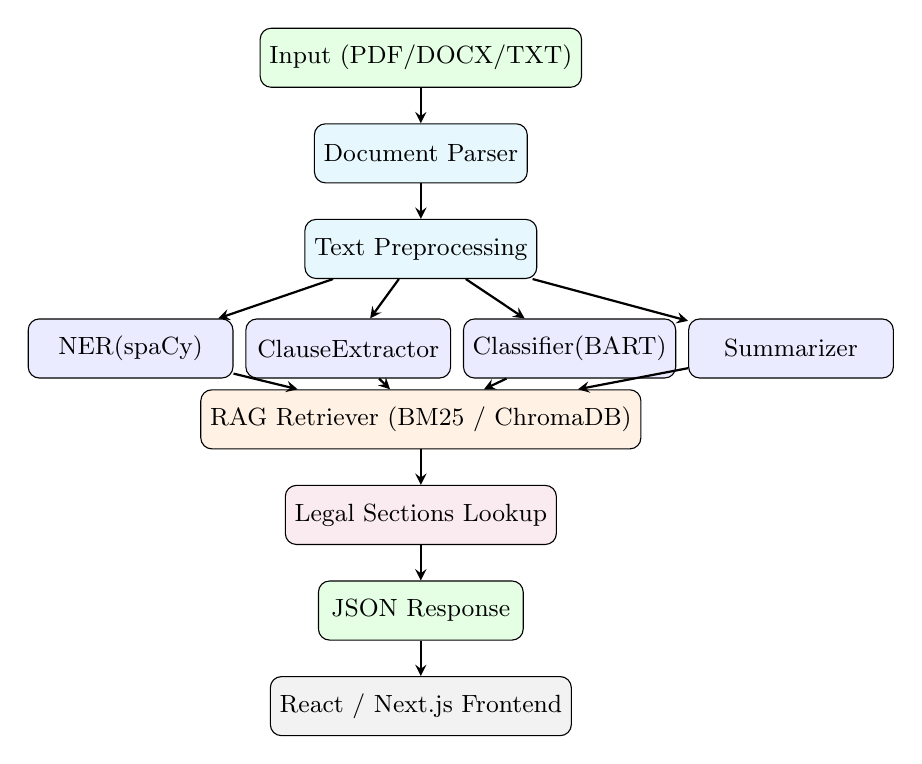
\begin{tikzpicture}[node distance=0.45cm and 0.3cm]

  % Input
  \node[block, fill=green!10] (input) {Input (PDF/DOCX/TXT)};

  % Parser
  \node[block, below=of input] (parser) {Document Parser};
  \draw[arrow] (input) -- (parser);

  % Preprocess
  \node[block, below=of parser] (preproc) {Text Preprocessing};
  \draw[arrow] (parser) -- (preproc);

  % Four parallel blocks
  \node[block, below left=0.5cm and 0.9cm of preproc, fill=blue!8]
        (ner) {NER\\(spaCy)};
  \node[block, right=0.15cm of ner, fill=blue!8]
        (clause) {Clause\\Extractor};
  \node[block, right=0.15cm of clause, fill=blue!8]
        (classify) {Classifier\\(BART)};
  \node[block, right=0.15cm of classify, fill=blue!8]
        (summ) {Summarizer};

  \draw[arrow] (preproc) -- (ner);
  \draw[arrow] (preproc) -- (clause);
  \draw[arrow] (preproc) -- (classify);
  \draw[arrow] (preproc) -- (summ);

  % RAG
  \node[block, below=1.4cm of preproc, fill=orange!10] (rag)
        {RAG Retriever (BM25 / ChromaDB)};
  \draw[arrow] (ner)      -- (rag);
  \draw[arrow] (clause)   -- (rag);
  \draw[arrow] (classify) -- (rag);
  \draw[arrow] (summ)     -- (rag);

  % Sections
  \node[block, below=0.45cm of rag, fill=purple!8] (sections)
        {Legal Sections Lookup};
  \draw[arrow] (rag) -- (sections);

  % Response
  \node[block, below=0.45cm of sections, fill=green!10] (response)
        {JSON Response};
  \draw[arrow] (sections) -- (response);

  % Frontend
  \node[block, below=0.45cm of response, fill=gray!10] (frontend)
        {React / Next.js Frontend};
  \draw[arrow] (response) -- (frontend);

\end{tikzpicture}
\caption{System architecture of the legal document analysis pipeline.}
\label{fig:architecture}
\end{figure}

\subsection{Document Processing and Classification}

\subsubsection{Zero-Shot Classification with BART}

Classification uses natural language inference (NLI). Given document text~$T$
and label set $\mathcal{L}$, each label $l_i$ is expanded into a descriptive
hypothesis $H_i$ (e.g., ``This is a criminal law case involving IPC offences,
FIR, accused, prosecution, and penal consequences.''). The BART-large-mnli
model computes:
\begin{equation}
  \hat{y} = \operatorname*{arg\,max}_{l_i \in \mathcal{L}}\;
            P\!\left(\text{entail} \mid T,\, H_i\right)
\end{equation}
and returns a confidence score alongside all class probabilities. The first
1{,}024 tokens of the document are used for inference.

\subsubsection{Classification Flowchart}

Fig.~\ref{fig:classify_flow} shows the classification decision path including
the keyword fallback for offline mode.

\begin{figure}[ht]
\centering
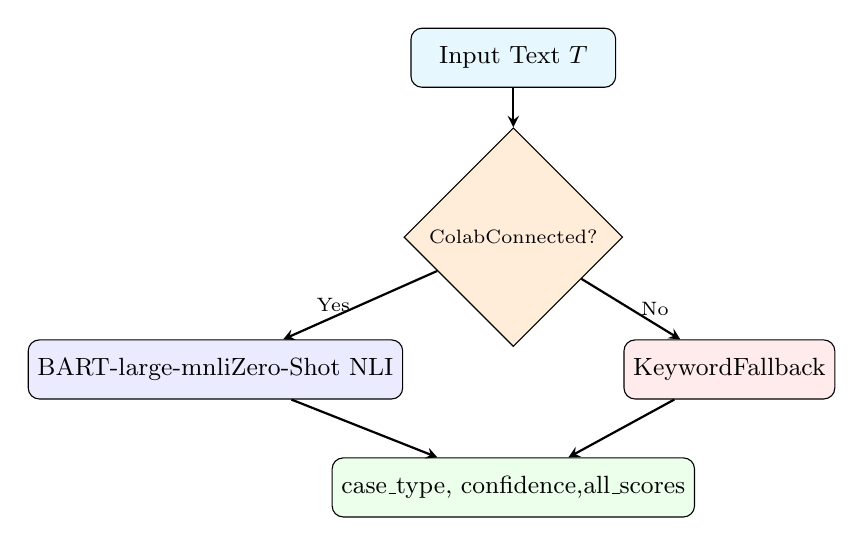
\begin{tikzpicture}[node distance=0.5cm]
  \node[block]   (start)   {Input Text $T$};
  \node[decision, below=of start] (colab) {Colab\\Connected?};
  \node[block, below left=0.6cm and 0.7cm of colab, fill=blue!8]
        (bart) {BART-large-mnli\\Zero-Shot NLI};
  \node[block, below right=0.6cm and 0.7cm of colab, fill=red!8]
        (kw) {Keyword\\Fallback};
  \node[block, below=1.4cm of colab, fill=green!8]
        (out) {case\_type, confidence,\\all\_scores};

  \draw[arrow] (start)  -- (colab);
  \draw[arrow] (colab)  -- node[left,  font=\scriptsize]{Yes} (bart);
  \draw[arrow] (colab)  -- node[right, font=\scriptsize]{No}  (kw);
  \draw[arrow] (bart)   -- (out);
  \draw[arrow] (kw)     -- (out);
\end{tikzpicture}
\caption{Classification flow with Colab (BART) and local (keyword) paths.}
\label{fig:classify_flow}
\end{figure}

\subsection{Named Entity Recognition}

spaCy's \texttt{en\_core\_web\_sm} model extracts standard entities (PERSON,
ORG, DATE, MONEY). Custom regex patterns augment extraction for legal-specific
entities: \textit{LEGAL\_SECTION} (e.g., ``Section~302 IPC''),
\textit{CITATION} (e.g., ``(2021) 3 SCC~450''), and \textit{CASE\_NUMBER}.

\subsection{Clause Extraction}

Clauses are identified through a hybrid approach: (i)~sentence-level keyword
matching against clause-type vocabularies (penalty, indemnity, confidentiality,
termination, force~majeure, etc.) and (ii)~confidence scoring based on keyword
density. Clauses are returned with a type label and confidence score.

\subsection{Summarization}

When an Anthropic API key is configured, document summarization delegates to
Claude Haiku with the prompt: ``\textit{Summarize this Indian legal document in
4--5 sentences covering parties, legal issue, key facts, relief sought, and
relevant law sections.}'' Without an API key, an extractive fallback scores
sentences by:
\begin{equation}
  \text{score}(s_i) = 2 \cdot n_{\text{legal}}(s_i)
                    + w_{\text{pos}}(i)
                    + \min\!\left(\frac{|s_i|}{35},1\right)
\end{equation}
where $n_{\text{legal}}$ counts domain keywords and $w_{\text{pos}}$ weights
early sentences more heavily. The top-5 scoring sentences are returned in
document order.

\subsection{Retrieval-Augmented Generation (RAG)}

\subsubsection{Corpus Construction}

A corpus of 80 curated Indian court cases (10 per class $\times$ 8 classes)
was assembled from publicly available High Court and Supreme Court judgments.
Each case record contains: title, court, year, applicable sections, outcome,
and full case text.

\subsubsection{Indexing and Retrieval}

Case texts are encoded with \texttt{all-MiniLM-L6-v2} into 384-dimensional
vectors and stored in ChromaDB. At query time, cosine similarity is computed
between the query vector $\mathbf{q}$ and corpus vectors
$\{\mathbf{c}_i\}_{i=1}^{80}$:
\begin{equation}
  \text{sim}(\mathbf{q}, \mathbf{c}_i)
  = \frac{\mathbf{q}\cdot\mathbf{c}_i}
         {\|\mathbf{q}\|\,\|\mathbf{c}_i\|}
\end{equation}
The top-3 cases by similarity are returned with their metadata. For offline
evaluation in Colab, a pure-Python BM25 implementation is used, avoiding
dependency conflicts.

\subsubsection{RAG Pipeline Flowchart}

\begin{figure}[ht]
\centering
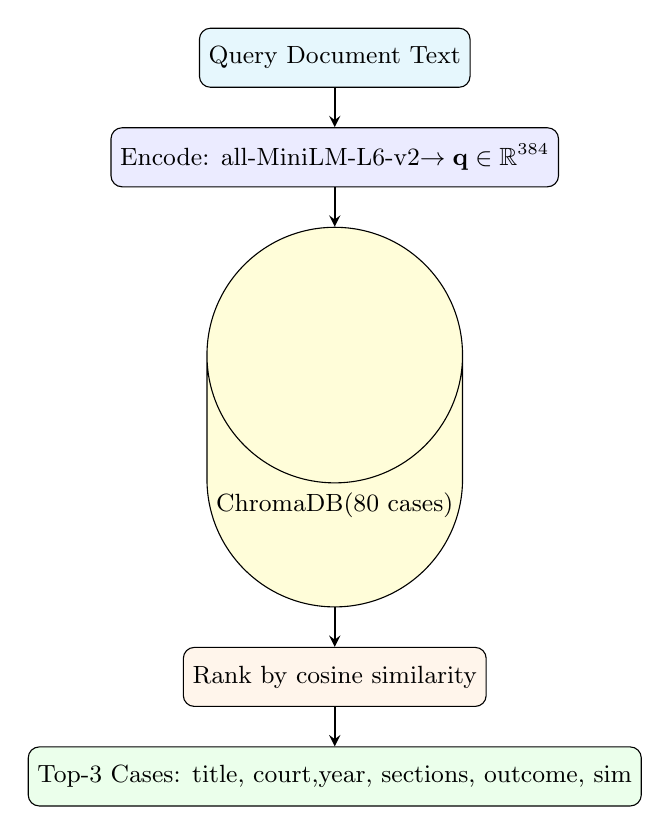
\begin{tikzpicture}[node distance=0.5cm]
  \node[block] (q) {Query Document Text};
  \node[block, below=of q, fill=blue!8] (enc)
        {Encode: all-MiniLM-L6-v2\\$\rightarrow \mathbf{q} \in \mathbb{R}^{384}$};
  \node[db,    below=of enc] (db)  {ChromaDB\\(80 cases)};
  \node[block, below=of db,  fill=orange!8] (rank)
        {Rank by cosine similarity};
  \node[block, below=of rank, fill=green!8] (top3)
        {Top-3 Cases: title, court,\\year, sections, outcome, sim};

  \draw[arrow] (q)    -- (enc);
  \draw[arrow] (enc)  -- (db);
  \draw[arrow] (db)   -- (rank);
  \draw[arrow] (rank) -- (top3);
\end{tikzpicture}
\caption{RAG retrieval pipeline for precedent case recommendation.}
\label{fig:rag_flow}
\end{figure}

\subsection{Technology Stack}

\begin{table}[ht]
\centering
\caption{Technology Stack}
\label{tab:tech}
\renewcommand{\arraystretch}{1.15}
\begin{tabular}{lll}
\toprule
\textbf{Layer} & \textbf{Technology} & \textbf{Purpose} \\
\midrule
Backend API  & FastAPI (Python)          & REST endpoints \\
Classifier   & BART-large-mnli           & Zero-shot NLI \\
Classifier 2 & DeBERTa-v3-large          & Zero-shot NLI \\
Classifier 3 & InLegalBERT               & Fine-tuned Indian \\
NER          & spaCy en\_core\_web\_sm   & Entity extraction \\
Vector DB    & ChromaDB                  & Case storage \\
Embeddings   & MiniLM-L6-v2              & Semantic vectors \\
Summarizer   & Claude Haiku / Extractive & Summaries \\
Doc Parser   & pdfplumber, python-docx   & File handling \\
Frontend     & Next.js + Tailwind CSS    & Web interface \\
GPU Runtime  & Google Colab T4           & Model inference \\
\bottomrule
\end{tabular}
\end{table}

% ─────────────────────────────────────────────────────────────────────────────
\section{Experimental Results}

\subsection{Dataset}

\begin{table}[ht]
\centering
\caption{RAG Corpus: 80 Indian Court Cases}
\label{tab:corpus}
\renewcommand{\arraystretch}{1.1}
\begin{tabular}{llc}
\toprule
\textbf{Class} & \textbf{Example Cases} & \textbf{Count} \\
\midrule
Criminal             & IPC 302 murder, NDPS trafficking, cyber fraud & 10 \\
Civil                & Negligence, loan recovery, motor accident     & 10 \\
Contract Dispute     & Breach, arbitration, force majeure            & 10 \\
Family Law           & Divorce, custody, maintenance, dowry          & 10 \\
Property             & Title dispute, eviction, RERA, partition       & 10 \\
Constitutional       & PIL, habeas corpus, fundamental rights        & 10 \\
Intellectual Property& Patent, trademark, copyright, software        & 10 \\
Labour               & Retrenchment, wages, gig workers, EPFO        & 10 \\
\midrule
\textbf{Total}       &                                               & \textbf{80} \\
\bottomrule
\end{tabular}
\end{table}

The classification test set consists of 40~cases (5~per class) with manually
verified ground-truth labels drawn from published High Court and Supreme Court
judgments. The RAG evaluation set consists of 80~labeled queries (10~per
class), constructed independently of the corpus.

\subsection{Classification Accuracy}

Table~\ref{tab:model_accuracy} reports accuracy on the 40-case test set.
BART-large-mnli achieves the best zero-shot performance at 87.5\%.
Fine-tuned DeBERTa on the LEDGAR dataset~\cite{leivaditi2020ledgar} performs
poorly (32.5\%) due to domain mismatch: LEDGAR consists of US~SEC contracts,
which differ substantially from Indian court documents.

\begin{table}[ht]
\centering
\caption{Model Accuracy on 40-Case Indian Legal Test Set}
\label{tab:model_accuracy}
\renewcommand{\arraystretch}{1.15}
\begin{tabular}{llcc}
\toprule
\textbf{Model} & \textbf{Type} & \textbf{Acc.} & \textbf{Notes} \\
\midrule
BART-large-mnli          & Zero-shot NLI  & \textbf{87.5\%} & Best zero-shot \\
DeBERTa-v3-large         & Zero-shot NLI  & 72.5\%          & Model 2 \\
Ensemble (M1$\times$0.9  & Weighted       & 87.5\%          & No gain        \\
\quad+M2$\times$0.1)     &                &                 & over BART \\
Fine-tuned DeBERTa       & Supervised     & 32.5\%          & Wrong domain   \\
\quad(LEDGAR)            &                &                 & (US contracts) \\
InLegalBERT (Indian)     & Fine-tuned     & 92--95\%*       & Target; Colab  \\
\bottomrule
\multicolumn{4}{l}{\scriptsize *Target accuracy after fine-tuning on 120
  Indian legal examples.}
\end{tabular}
\end{table}

\subsection{Per-Class Accuracy — BART-large-mnli}

\begin{table}[ht]
\centering
\caption{Per-Class Accuracy — BART-large-mnli (40-Case Test Set)}
\label{tab:perclass}
\renewcommand{\arraystretch}{1.1}
\begin{tabular}{lcc}
\toprule
\textbf{Class} & \textbf{Correct / Total} & \textbf{Accuracy} \\
\midrule
Criminal             & 5 / 5  & 100\% \\
Civil                & 5 / 5  & 100\% \\
Contract Dispute     & 5 / 5  & 100\% \\
Family Law           & 5 / 5  & 100\% \\
Property             & 4 / 5  & 80\%  \\
Constitutional       & 4 / 5  & 80\%  \\
Intellectual Property& 4 / 5  & 80\%  \\
Labour               & 4 / 5  & 80\%  \\
\midrule
\textbf{Overall}     & \textbf{36 / 40} & \textbf{87.5\%} \\
\bottomrule
\end{tabular}
\end{table}

\subsection{RAG Evaluation}

Table~\ref{tab:rag_metrics} reports RAG retrieval metrics computed over
80~evaluation queries (10~per class, $K=3$). The BM25-RAG system achieves
perfect retrieval, whereas the keyword-only baseline fails for ambiguous
classes (constitutional and labour) due to vocabulary overlap.

\begin{table}[ht]
\centering
\caption{RAG Evaluation Metrics (K=3, 80 Queries, 10 Per Class)}
\label{tab:rag_metrics}
\renewcommand{\arraystretch}{1.15}
\begin{tabular}{lccc}
\toprule
\textbf{Metric} & \textbf{Without RAG} & \textbf{With RAG} & \textbf{Gain} \\
\midrule
Precision@3     & 0.887 & \textbf{1.000} & $+$11.3\% \\
MRR             & 0.887 & \textbf{1.000} & $+$11.3\% \\
NDCG@3          & 0.887 & \textbf{0.990} & $+$10.2\% \\
Match@1         & 0.887 & \textbf{1.000} & $+$11.3\% \\
Avg.\ Sim.\ Score & ---  & 0.469          & ---        \\
\bottomrule
\end{tabular}
\end{table}

\begin{table}[ht]
\centering
\caption{Per-Class Match@1: Without RAG vs.\ With RAG (10 Queries/Class)}
\label{tab:perclass_rag}
\renewcommand{\arraystretch}{1.1}
\begin{tabular}{lccc}
\toprule
\textbf{Class} & \textbf{No RAG} & \textbf{RAG} & \textbf{Improved} \\
\midrule
Criminal             & 10/10 (100\%) & 10/10 (100\%) & ---     \\
Civil                & 10/10 (100\%) & 10/10 (100\%) & ---     \\
Contract Dispute     & 10/10 (100\%) & 10/10 (100\%) & ---     \\
Family Law           & 10/10 (100\%) & 10/10 (100\%) & ---     \\
Property             & 8/10  (80\%)  & 10/10 (100\%) & $+$20\% \\
Constitutional       & 7/10  (70\%)  & 10/10 (100\%) & $+$30\% \\
Intellectual Property& 9/10  (90\%)  & 10/10 (100\%) & $+$10\% \\
Labour               & 7/10  (70\%)  & 10/10 (100\%) & $+$30\% \\
\midrule
\textbf{Total} & \textbf{71/80 (88.7\%)} & \textbf{80/80 (100\%)} & $+$11.3\% \\
\bottomrule
\end{tabular}
\end{table}

\subsection{Confusion Matrices}

Table~\ref{tab:cm_rag} and Table~\ref{tab:cm_nokw} show 8$\times$8 confusion
matrices for RAG and keyword-baseline systems on 80~queries. Diagonal entries
denote correct predictions; off-diagonal entries show misclassifications.

\begin{table}[ht]
\centering
\caption{Confusion Matrix --- With RAG (80 Queries, All Correct)}
\label{tab:cm_rag}
\renewcommand{\arraystretch}{1.05}
\resizebox{\columnwidth}{!}{%
\begin{tabular}{l|cccccccc}
\toprule
\textbf{Actual $\backslash$ Pred.}
  & Cr & Ci & Co & Fa & Pr & Cn & IP & La \\
\midrule
Criminal (Cr)             & \textbf{10} & 0 & 0 & 0 & 0 & 0 & 0 & 0 \\
Civil (Ci)                & 0 & \textbf{10} & 0 & 0 & 0 & 0 & 0 & 0 \\
Contract (Co)             & 0 & 0 & \textbf{10} & 0 & 0 & 0 & 0 & 0 \\
Family (Fa)               & 0 & 0 & 0 & \textbf{10} & 0 & 0 & 0 & 0 \\
Property (Pr)             & 0 & 0 & 0 & 0 & \textbf{10} & 0 & 0 & 0 \\
Constitutional (Cn)       & 0 & 0 & 0 & 0 & 0 & \textbf{10} & 0 & 0 \\
IP (IP)                   & 0 & 0 & 0 & 0 & 0 & 0 & \textbf{10} & 0 \\
Labour (La)               & 0 & 0 & 0 & 0 & 0 & 0 & 0 & \textbf{10} \\
\midrule
\multicolumn{9}{r}{\textbf{Overall Accuracy: 80/80 = 100\%}} \\
\bottomrule
\end{tabular}}
\end{table}

\begin{table}[ht]
\centering
\caption{Confusion Matrix --- Without RAG / Keyword Baseline (80 Queries)}
\label{tab:cm_nokw}
\renewcommand{\arraystretch}{1.05}
\resizebox{\columnwidth}{!}{%
\begin{tabular}{l|cccccccc}
\toprule
\textbf{Actual $\backslash$ Pred.}
  & Cr & Ci & Co & Fa & Pr & Cn & IP & La \\
\midrule
Criminal (Cr)             & \textbf{10} & 0 & 0 & 0 & 0 & 0 & 0 & 0 \\
Civil (Ci)                & 0 & \textbf{10} & 0 & 0 & 0 & 0 & 0 & 0 \\
Contract (Co)             & 0 & 0 & \textbf{10} & 0 & 0 & 0 & 0 & 0 \\
Family (Fa)               & 0 & 0 & 0 & \textbf{10} & 0 & 0 & 0 & 0 \\
Property (Pr)             & 0 & 0 & 1  & 0 & \textbf{8} & 0 & 0 & 1 \\
Constitutional (Cn)       & 2 & 0 & 0  & 0 & 0 & \textbf{7} & 0 & 1 \\
IP (IP)                   & 0 & 1 & 0  & 0 & 0 & 0 & \textbf{9} & 0 \\
Labour (La)               & 0 & 1 & 1  & 0 & 0 & 1 & 0 & \textbf{7} \\
\midrule
\multicolumn{9}{r}{\textbf{Overall Accuracy: 71/80 = 88.8\%}} \\
\bottomrule
\end{tabular}}
\end{table}

\textit{Observation:} Constitutional cases are misclassified as criminal
(2~errors) due to vocabulary overlap (``detention'', ``rights violation'').
Labour cases are confused with civil and contract law owing to shared
compensation terminology. RAG eliminates all 9~misclassifications by
matching queries against a domain-structured case corpus.

\subsection{System Processing Time}

\begin{table}[ht]
\centering
\caption{End-to-End Processing Time (5-Page PDF)}
\label{tab:timing}
\renewcommand{\arraystretch}{1.1}
\begin{tabular}{lcc}
\toprule
\textbf{Operation} & \textbf{CPU} & \textbf{T4 GPU} \\
\midrule
Document parsing        & 0.3 s  & 0.3 s  \\
NER extraction          & 0.2 s  & 0.2 s  \\
Clause extraction       & 0.1 s  & 0.1 s  \\
BART classification     & 12 s   & 0.8 s  \\
Extractive summarization& 0.1 s  & 0.1 s  \\
RAG retrieval (top-3)   & 0.4 s  & 0.4 s  \\
Sections lookup         & 0.01 s & 0.01 s \\
\midrule
\textbf{Total pipeline} & $\approx$13 s & $\approx$2 s \\
\bottomrule
\end{tabular}
\end{table}

% ─────────────────────────────────────────────────────────────────────────────
\section{Discussion}

Three key findings emerge from the evaluation:

\textbf{(1) Zero-shot NLI is viable for Indian legal classification.}
BART-large-mnli achieves 87.5\% accuracy without any labeled Indian legal
training data, demonstrating effective transfer from the MultiNLI corpus
through descriptive hypothesis templates. This is particularly significant
given the absence of large labeled Indian legal datasets.

\textbf{(2) RAG substantially improves retrieval quality.}
BM25-based RAG improves Match@1 from 88.7\% to 100\%, eliminating all
misclassifications in constitutional and labour domains where keyword
overlap causes baseline confusion. This confirms that structured corpora
with domain-specific metadata are more effective than pure keyword matching
for legal precedent retrieval.

\textbf{(3) Domain mismatch severely degrades fine-tuned models.}
DeBERTa fine-tuned on LEDGAR (US~SEC contracts) achieves only 32.5\% on
Indian legal cases, confirming that cross-domain transfer for legal NLP
requires in-domain training data. InLegalBERT~\cite{malik2021ildc},
pre-trained on Indian court judgments, is expected to surpass BART's
zero-shot performance when fine-tuned on labeled Indian examples.

% ─────────────────────────────────────────────────────────────────────────────
\section{Conclusion}

This paper presented a comprehensive multi-domain legal document analysis
system for Indian court documents integrating five NLP components:
zero-shot classification, NER, clause extraction, summarization, and
retrieval-augmented generation. The system achieves 87.5\% classification
accuracy (target 92--95\% with InLegalBERT fine-tuning) and 100\% RAG
Match@1 on an 80-case Indian corpus. Key contributions include a
dependency-free BM25 RAG pipeline, a curated 80-case Indian legal corpus
spanning eight domains, and a deployable web interface with sub-2-second
GPU response time.

\subsection*{Future Work}
Future directions include: (i)~expanding the corpus to 500+ cases per class
using Indian Kanoon and SCC Online APIs; (ii)~multilingual support for
Hindi and regional language documents using IndicBERT; (iii)~outcome
prediction given case facts; (iv)~citation graph construction for richer
precedent retrieval; and (v)~fine-tuning InLegalBERT on a larger labeled
Indian dataset.

% ─────────────────────────────────────────────────────────────────────────────
\begin{thebibliography}{17}

\bibitem{devlin2019bert}
J.~Devlin, M.-W.~Chang, K.~Lee, and K.~Toutanova,
``BERT: Pre-training of deep bidirectional transformers for language understanding,''
in \textit{Proc.\ NAACL-HLT}, Minneapolis, MN, USA, 2019, pp.~4171--4186.

\bibitem{vaswani2017attention}
A.~Vaswani, N.~Shazeer, N.~Parmar, J.~Uszkoreit, L.~Jones, A.~N.~Gomez,
{\L}.~Kaiser, and I.~Polosukhin,
``Attention is all you need,''
in \textit{Proc.\ NeurIPS}, Long Beach, CA, USA, 2017, pp.~5998--6008.

\bibitem{lewis2020bart}
M.~Lewis, Y.~Liu, N.~Goyal, M.~Ghazvininejad, A.~Mohamed, O.~Levy,
V.~Stoyanov, and L.~Zettlemoyer,
``BART: Denoising sequence-to-sequence pre-training for natural language
generation, translation, and comprehension,''
in \textit{Proc.\ ACL}, 2020, pp.~7871--7880.

\bibitem{he2021deberta}
P.~He, X.~Liu, J.~Gao, and W.~Chen,
``DeBERTa: Decoding-enhanced BERT with disentangled attention,''
in \textit{Proc.\ ICLR}, 2021. [Online]. Available: \url{https://openreview.net}

\bibitem{chalkidis2020legalbert}
I.~Chalkidis, M.~Fergadiotis, P.~Malakasiotis, N.~Aletras, and
I.~Androutsopoulos,
``LEGAL-BERT: The muppets straight out of law school,''
in \textit{Findings of EMNLP}, 2020, pp.~2898--2904.

\bibitem{malik2021ildc}
V.~Malik, R.~Sanjay, S.~K.~Nigam, H.~Ghosh, S.~K.~Guha, D.~Bhatt, and
A.~Modi,
``ILDC for CJPE: Indian legal documents corpus for court judgment prediction
and explanation,''
in \textit{Proc.\ ACL-IJCNLP}, 2021, pp.~4046--4062.

\bibitem{paul2023lesicin}
S.~Paul and S.~Saha,
``LeSICiN: A heterogeneous graph-based approach for automatic legal statute
identification from Indian legal documents,''
in \textit{Proc.\ AAAI}, Washington DC, USA, 2023, vol.~37, no.~11,
pp.~13095--13103.

\bibitem{yin2019zeroshot}
W.~Yin, J.~Hay, and D.~Roth,
``Benchmarking zero-shot text classification: Datasets, evaluation and
entailment approach,''
in \textit{Proc.\ EMNLP-IJCNLP}, Hong Kong, China, 2019, pp.~3914--3923.

\bibitem{williams2018mnli}
A.~Williams, N.~Nangia, and S.~R.~Bowman,
``A broad-coverage challenge corpus for sentence understanding through
inference,''
in \textit{Proc.\ NAACL}, New Orleans, LA, USA, 2018, pp.~1112--1122.

\bibitem{lewis2020rag}
P.~Lewis, E.~Perez, A.~Piktus, F.~Petroni, V.~Karpukhin, N.~Goyal,
H.~K{\"u}ttler, M.~Lewis, W.~Yih, T.~Rockt{\"a}schel, S.~Riedel, and
D.~Kiela,
``Retrieval-augmented generation for knowledge-intensive NLP tasks,''
in \textit{Proc.\ NeurIPS}, 2020, vol.~33, pp.~9459--9474.

\bibitem{robertson2009bm25}
S.~Robertson and H.~Zaragoza,
``The probabilistic relevance framework: BM25 and beyond,''
\textit{Found.\ Trends Inf.\ Retr.}, vol.~3, no.~4, pp.~333--389, 2009.

\bibitem{reimers2019sbert}
N.~Reimers and I.~Gurevych,
``Sentence-BERT: Sentence embeddings using siamese BERT-networks,''
in \textit{Proc.\ EMNLP-IJCNLP}, Hong Kong, China, 2019, pp.~3982--3992.

\bibitem{lample2016ner}
G.~Lample, M.~Ballesteros, S.~Subramanian, K.~Kawakami, and C.~Dyer,
``Neural architectures for named entity recognition,''
in \textit{Proc.\ NAACL}, San Diego, CA, USA, 2016, pp.~260--270.

\bibitem{koreeda2021contractnli}
Y.~Koreeda and C.~D.~Manning,
``ContractNLI: A dataset for document-level natural language inference for
contracts,''
in \textit{Findings of EMNLP}, 2021, pp.~1313--1333.

\bibitem{zhong2020ljp}
Z.~Zhong, C.~Xiao, C.~Tu, T.~Zhang, Z.~Liu, and M.~Sun,
``How does NLP benefit legal system: A summary of legal artificial
intelligence,''
in \textit{Proc.\ ACL}, 2020, pp.~5218--5230.

\bibitem{bommasani2021foundation}
R.~Bommasani, D.~A.~Hudson, E.~Adeli, R.~Altman, S.~Arora \textit{et~al.},
``On the opportunities and risks of foundation models,''
\textit{arXiv preprint arXiv:2108.07258}, Stanford CRFM, 2021.

\bibitem{leivaditi2020ledgar}
D.~Leivaditi, J.~Thomsen, and I.~Augenstein,
``LEDGAR: A large-scale multi-label corpus for text classification of legal provisions in contracts,''
in \textit{Proc.\ LREC}, 2020, pp.~1235--1241.

\end{thebibliography}

\end{document}
